%%%%%%%%%%%%%%%%%%%%%%%%%%%%%%%%%%%%%%%%%
% Beamer Presentation
% LaTeX Template
% Version 1.0 (10/11/12)
%
% This template has been downloaded from:
% http://www.LaTeXTemplates.com
%
% License:
% CC BY-NC-SA 3.0 (http://creativecommons.org/licenses/by-nc-sa/3.0/)
%
%%%%%%%%%%%%%%%%%%%%%%%%%%%%%%%%%%%%%%%%%

%----------------------------------------------------------------------------------------
%	PACKAGES AND THEMES
%----------------------------------------------------------------------------------------

\documentclass[compress]{beamer}

\mode<presentation> {

% The Beamer class comes with a number of default slide themes
% which change the colors and layouts of slides. Below this is a list
% of all the themes, uncomment each in turn to see what they look like.

%\usetheme{default}
%\usetheme{AnnArbor}
%\usetheme{Antibes}
%\usetheme{Bergen}
%\usetheme{Berkeley}
\usetheme{Berlin}
%\usetheme{Boadilla}
%\usetheme{CambridgeUS}
%\usetheme{Copenhagen}
%\usetheme{Darmstadt}
%\usetheme{Dresden}
%\usetheme{Frankfurt}
%\usetheme{Goettingen}
%\usetheme{Hannover}
%\usetheme{Ilmenau}
%\usetheme{JuanLesPins}
%\usetheme{Luebeck}
%\usetheme{Madrid}
%\usetheme{Malmoe}
%\usetheme{Marburg}
%\usetheme{Montpellier}
%\usetheme{PaloAlto}
%\usetheme{Pittsburgh}
%\usetheme{Rochester}
%\usetheme{Singapore}
%\usetheme{Szeged}
%\usetheme{Warsaw}

% As well as themes, the Beamer class has a number of color themes
% for any slide theme. Uncomment each of these in turn to see how it
% changes the colors of your current slide theme.

%\usecolortheme{albatross}
%\usecolortheme{beaver}
%\usecolortheme{beetle}
%\usecolortheme{crane}
%\usecolortheme{dolphin}
%\usecolortheme{dove}
%\usecolortheme{fly}
%\usecolortheme{lily}
%\usecolortheme{orchid}
%\usecolortheme{rose}
%\usecolortheme{seagull}
%\usecolortheme{seahorse}
%\usecolortheme{whale}
%\usecolortheme{wolverine}

%\setbeamertemplate{footline} % To remove the footer line in all slides uncomment this line
\setbeamertemplate{footline}[page number] % To replace the footer line in all slides with a simple slide count uncomment this line

%\setbeamertemplate{navigation symbols}{} % To remove the navigation symbols from the bottom of all slides uncomment this line
}

\usepackage{graphicx} % Allows including images
\usepackage{booktabs} % Allows the use of \toprule, \midrule and \bottomrule in tables
\usepackage{color}
\usepackage{mathrsfs}
\usepackage{type1cm}
\newcommand{\ty}{\fontsize{4pt}{6pt}\selectfont}
\setbeamertemplate{caption}[numbered]

% image directory
\graphicspath{{imgs/}}

% font
\usepackage{times}
\usefonttheme{professionalfonts}

% caption font size
\usepackage{caption}
\captionsetup{font={small}}

\usepackage{comment}
\usepackage{multirow}

\hypersetup{
  pdfauthor={Liu Weizhi},
  pdfpagemode=FullScreen,
  colorlinks={true}
}
%----------------------------------------------------------------------------------------
%	TITLE PAGE
%----------------------------------------------------------------------------------------

\title[CS5330 Project]{Mazimizing Network Reward \\ Based on A General Framework of \\ Monte Carlo Tree Search} % The short title appears at the bottom of every slide, the full title is only on the title page

\author{Liu Weizhi} % Your name
\institute[NUS - ISE] % Your institution as it will appear on the bottom of every slide, may be shorthand to save space
{
Department of Industrial \& Systems Engineering \\ National University of Singapore \\ % Your institution for the title page
\medskip
\textit{weizhiliu2009@gmail.com} % Your email address
}
\date{\today} % Date, can be changed to a custom date

\begin{document}
\small

\begin{frame}
\titlepage % Print the title page as the first slide
\end{frame}

\begin{frame}
\frametitle{Overview} % Table of contents slide, comment this block out to remove it
\tableofcontents % Throughout your presentation, if you choose to use \section{} and \subsection{} commands, these will automatically be printed on this slide as an overview of your presentation
\end{frame}

%----------------------------------------------------------------------------------------
%	PRESENTATION SLIDES
%----------------------------------------------------------------------------------------
\section{Introduction}
\subsection{Task}
\begin{frame}
              \begin{itemize}
                \item Game Rule
                   \begin{itemize}
                     \item Input: undirected network adjacency list and original color sequence
                     \item Initial: choose a node whatever you like and color it
                     \item Process: pick a node from those uncolored nodes which connect to colored nodes and color it 
                     \item Terminate: the original color sequence runs out or no further candidate nodes to color
                     \item Reward: number of edges which connect to two different color nodes
                     \item Output: population sequence and network reward                       
                   \end{itemize}
                \item Goal: search the optimal network population sequence in order to maximize the total reward of the network
              \end{itemize}
\end{frame}
%----------------------------------------------------------------------------------------

\subsection{Challenge \& Solution}
\begin{frame}
\begin{itemize}
  \item Challenge
    \begin{itemize}
      \item Naive brute force algorithm could consume enormous computation budget when the network is large enough.
      \item Monte Carlo Tree Search algorithms might be a possible and efficient way.
      \item However, there exists various MCTS algorithms. So which algorithm might be useful for this specified project?
    \end{itemize}
  \item Solution
    \begin{itemize}
      \item \textit{\textbf{Monte carlo search algorithm discovery for one player games (Francis Maes et. al 2012)}}
      \item Generate abundant potential MCTS algorithms by combining basic search components. 
      \item {\color{red}Select the most appropriate algorithm generated for this specified project and then search the optimal population sequence. }
    \end{itemize}
\end{itemize}
\end{frame}

\section{Methods}

\subsection{Notations}

\begin{frame}
\begin{table}[htbp]
  \tiny
  \centering
  \caption{Notations}
    \begin{tabular}{cc}
    \toprule
    notation &  definition \\
    \midrule
    {\color{red}$\mathcal{A}_{n \times n}$} & adjacent matrix of the network with $n$ nodes\\
    $a_{ij}$ & element of $\mathcal{A}_{n \times n}$ which represents the number of edges between node $i$ and $j$ \\
    $\vec s$ & the original input sequence \\
    {\color{red}$\vec c_{1 \times n}$} & color vector for every nodes, $c_{i}$ represents the color of node $i$\\
    {\color{red}$r_{ij}$} & reward value between node $i$ and node $j$\\
    {\color{red}$R(\mathcal{A}_{n \times n}, \vec c_{1 \times n})$} & total reward of the network \\
    $R^{*}$ & current best network reward \\
   {\color{red} $w_{k}$} & the candidate nodes set at step $k$\\
    {\color{red}$\vec p_{k} = (p_{1}, p_{2}, \cdots, p_{k})$} & population sequence at step $k$ of which element $p_{i}$ represents the $i$th populated nodes\\
    $\vec p^{*}$ & current best population sequence \\
    $\tau(k)$ & represents if the game enters into end at time $k$\\
    $B$ & total budget for each algorithm \\
    $numCalls$ & current times of evaluation \\
    $\mathcal{S}$ & search component \\
    $N^{(repeat)}$ & repeat times for repeat component \\
    {\color{red}$N^{(select)}$} & multiple factor for select component \\
    $\eta$ & weight factor for exploring of ucb value \\
    $\mathcal{L}_{i}$ & the lower level search component standalone parameters recursive list at level $i$\\
    \bottomrule
    \end{tabular}%
  \label{tab:notations}%
\end{table}%
\end{frame}

\subsection{Network Construction and Reward Evaluation}
\begin{frame}
\begin{itemize}
  \item Network Construction: The network $\mathcal{A}_{n \times n}$ could be constructed based on the network adjacent list by continuously update $a_{ij}$ (number of edges between node $i$ and $j$). 
  \item Reward Evaluation
    \begin{itemize}
      \item Redefine Color Sequence $\vec c_{1 \times n}$:
\begin{align}
  c_{i} = \left \{
             \begin{array}{cl}
               -1 & \mbox{if node $i$'s color is 0} \\
               0 & \mbox{if node $i$ is not colored} \\
               1 & \mbox{if node $i$'s color is 1} \\
             \end{array}
          \right.
\end{align}

      \item Reward Calculation based on Matrix
        
\begin{equation}
\begin{aligned}
  r_{ij} = \frac{(c_{i}c_{j} - 1)}{2} c_{i} c_{j} a_{ij} = \frac{1}{2} (c_{i}^{2}a_{ij}c_{j}^{2} - c_{j}a_{ij}c_{j})
\end{aligned}
\end{equation}

\begin{equation}
\begin{aligned}
  R(\mathcal{A}, \vec c) =  \frac{1}{2} \sum_{i} \sum_{j} r_{ij} = \frac{1}{4} [(\vec c)^{2} \mathcal{A} (\vec c^{T})^{2} - \vec c \mathcal{A} \vec c^{T}]
\end{aligned}
\end{equation} 
    \end{itemize}
\end{itemize}
\end{frame}

\subsection{General Framework of MCTS}

\begin{frame}
\frametitle{Helper Components}
\begin{table}[htbp]
  \centering
  \tiny
  \caption{Illustration of helper components}
    \begin{tabular}{cccc}
    \toprule
    helper component &  task  & input & output \\
    \midrule
    candidate & update candidate nodes set for populating & $\vec p_{k-1}, p_{k}, w_{k-1}$ & $w_{k}$\\
     & by set operation rather than loop& & \\
    terminal & check wheter the game enters into end & $\vec p_{k}, w_{k}$ & $\tau(k)$ \\
    reward & calculate the network reward & $\mathcal{A}_{n \times n}, \vec c_{1 \times n}$ & R\\
    evaluate & update the budget consumption, best & $\vec p_{k}, \vec p^{*}, R^{*}, \mathcal{A}_{n \times n}, \vec c_{1 \times n}$ & $\vec p^{*}, R^{*}, $\\
      & reward and population sequence & $numCalls, B$ & $ numCalls$ \\
    invoke & invoke other search components & $\vec p_{k}, w_{k}, \mathcal{S}$ & $\vec p_{m} (m > k)$ \\
    \bottomrule
    \end{tabular}%
  \label{tab:helper_components}%
\end{table}%
\end{frame}

\begin{frame}
\frametitle{Search Components}
\begin{itemize}
  \item Two types of search components: atom component and free component
  \item free component can invoke other search components
  \item atom component can only be invoked by other search components
\end{itemize}
\begin{table}[htbp]
  \tiny
  \centering
  \caption{Illustration of search components}
    \begin{tabular}{ccc}
    \toprule
    search component &  task & type\\
    \midrule
    simulate & uniformly randomly select a full population sequence & atom component\\
    step & generate a full population sequence step by step & free component\\
    repeat & return the best population by repeating $N^{repeat}$ times evaluation & free component\\
    lookahead & return the best population by evaluating full population &  \\
    & sequence among all next candidates & free component\\
    select & a mini version of UCB & free component\\
    \bottomrule
    \end{tabular}%
  \label{tab:search_components}%
\end{table}%xs
\end{frame}

\begin{frame}
\frametitle{Search Components}
There are basically two major differences for select component from Maes.
\begin{itemize}
  \item Budget automatic adjustment
    \begin{equation}
    \begin{aligned}
      Budget(k)^{select} & = \\
      Size(w_{k}) & [(1 - \frac{Dim(\mathcal{A}) N^{select}}{Size(w_{k})}) \frac{Size(\vec p_{k})}{Size(\vec s)} + \frac{Dim(\mathcal{A}) N^{select}}{Size(w_{k})}] \\ 
    \end{aligned}
    \end{equation}
  \item Normalization for UCB value \\
    \begin{itemize}
      \item The reward part and explore part is extremely different in terms of scale.
      \item Divide reward part by the current best reward.
      \item Transform explore part into $(0,1)$ via logistic function.
      \item {\color{red}However, the search space is too large that explore too much may not be a good choice.}
    \end{itemize}
\end{itemize}
\end{frame}

\begin{frame}
\frametitle{Algorithms Generator}
\begin{table}[htbp]
  \centering
  \scriptsize
  \caption{MCTS algorithms examples}
    \begin{tabular}{cc}
    \toprule
    algorithm & recursive expression\\
    \midrule
    rmc($N_{1}^{select}, N_{2}^{select}$) & step(repeat($N_{1}^{select}$, step(repeat($N_{2}^{select}$, simulate()))))\\
    nmc(1) & step(lookahead(simulate())) \\
    nmc(2) & step(lookahead(step(lookahead(simulate())))) \\
    uct($N^{repeat}, N^{select}, \eta$) & step(repeat($N^{repeat}$, select($N^{select}, \eta$, simulate())))\\
    \bottomrule
    \end{tabular}%
  \label{tab:algo_examples}%
\end{table}%xs
\end{frame}

\section{Results \& Discussion}

\subsection{Datasets}

\begin{frame}
A possible simulation path should be set 1, set 2, set 3, set 6, set 4, set 5 and set 7 considering the difficulity of different datasets.
\begin{table}[htbp]
  \centering
  \caption{Descriptions of datasets}
    \begin{tabular}{ccc}
    \toprule
    dataset & network size (range) & sequence size \\
    \midrule
    set 1 & 10 & 10 \\
    set 2 & 153 & 20 \\
    set 3 & 153 & 130 \\
    set 4 & 961 & 400 \\
    set 5 & 5002 & 4000 \\
    set 6 & 483 & 400 \\
    set 7 & 11748 & 9000 \\
    \bottomrule
    \end{tabular}%
  \label{tab:datasets}%
\end{table}%
\end{frame}

\subsection{Algorithms Comparision}

\begin{frame}
\frametitle{Optimality and Efficiency}
In order to find the most suitable MCTS algorithm for this project,10000 budget are allocated to each algorithm and 10 independent simulation runs are conducted.
\begin{columns}
\column{.5\textwidth}
\begin{figure}[htbp!]
\centering
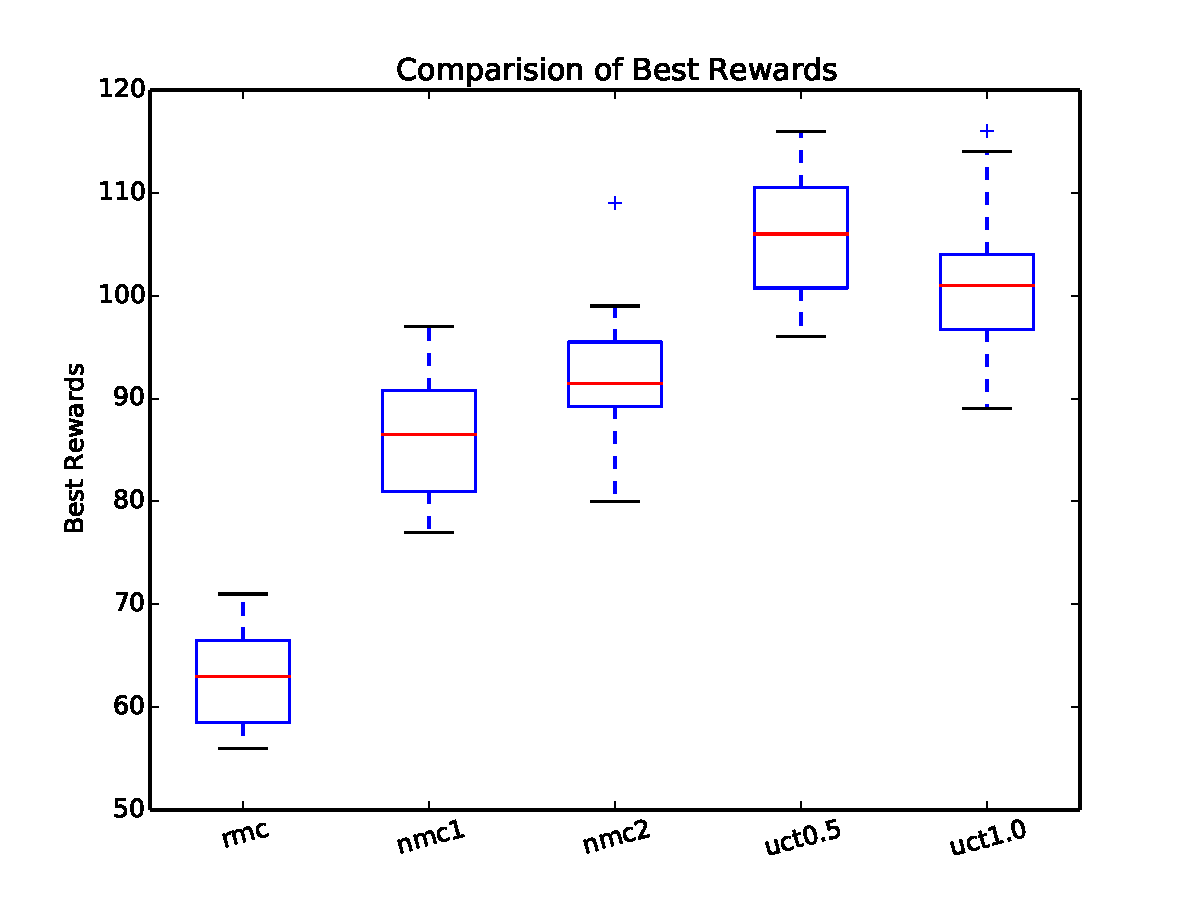
\includegraphics[width=1.0\textwidth]{best_reward_compare.pdf}
\caption{\label{fig:optimality}Best Rewards}
\end{figure}
\column{.5\textwidth}
\begin{figure}[htbp!]
\centering
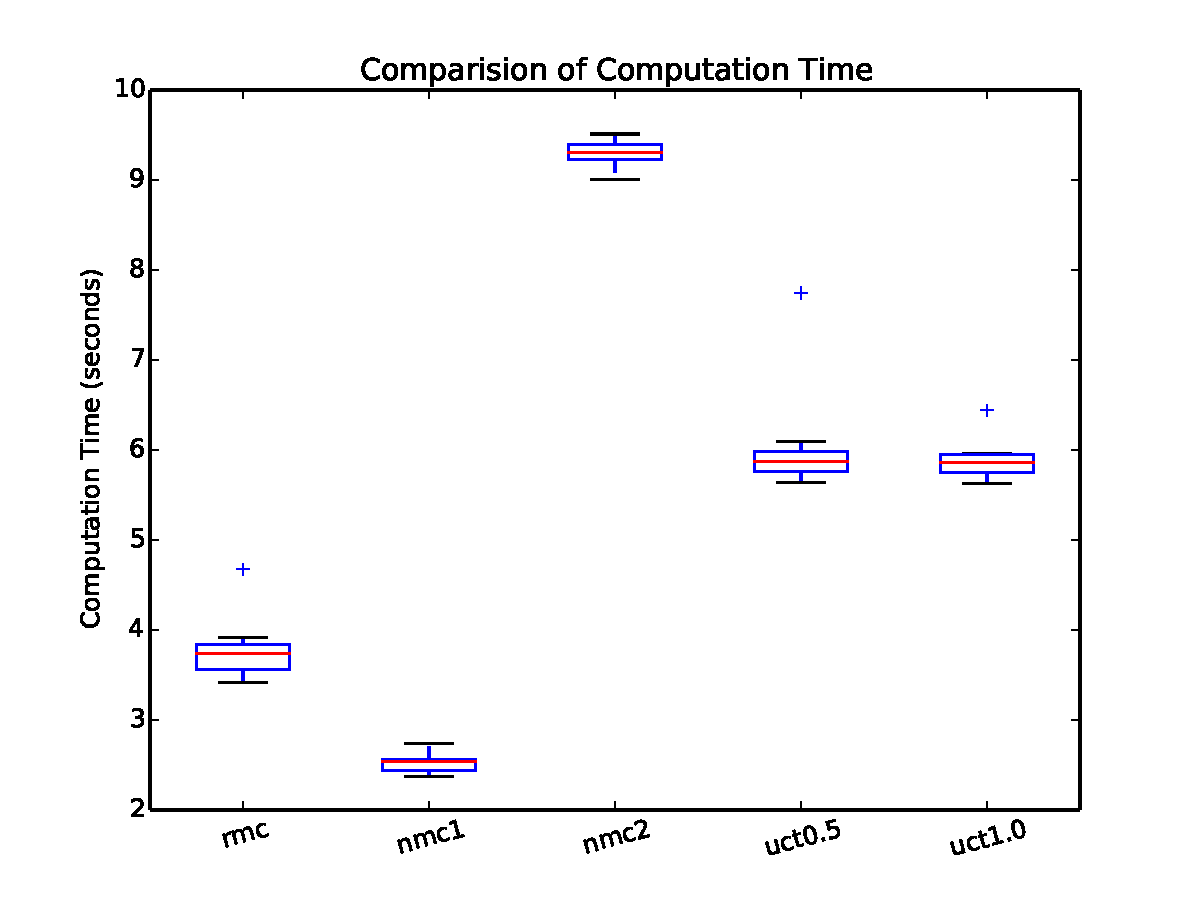
\includegraphics[width=1.0\textwidth]{computation_time_compare.pdf}
\caption{\label{fig:computation_time}Computation Time}
\end{figure}
\end{columns}
Apparently, uct is most suitable for this project comparing with any other popular MCTS algorithms 
\end{frame}

\begin{frame}
\begin{figure}[htb!]
\centering
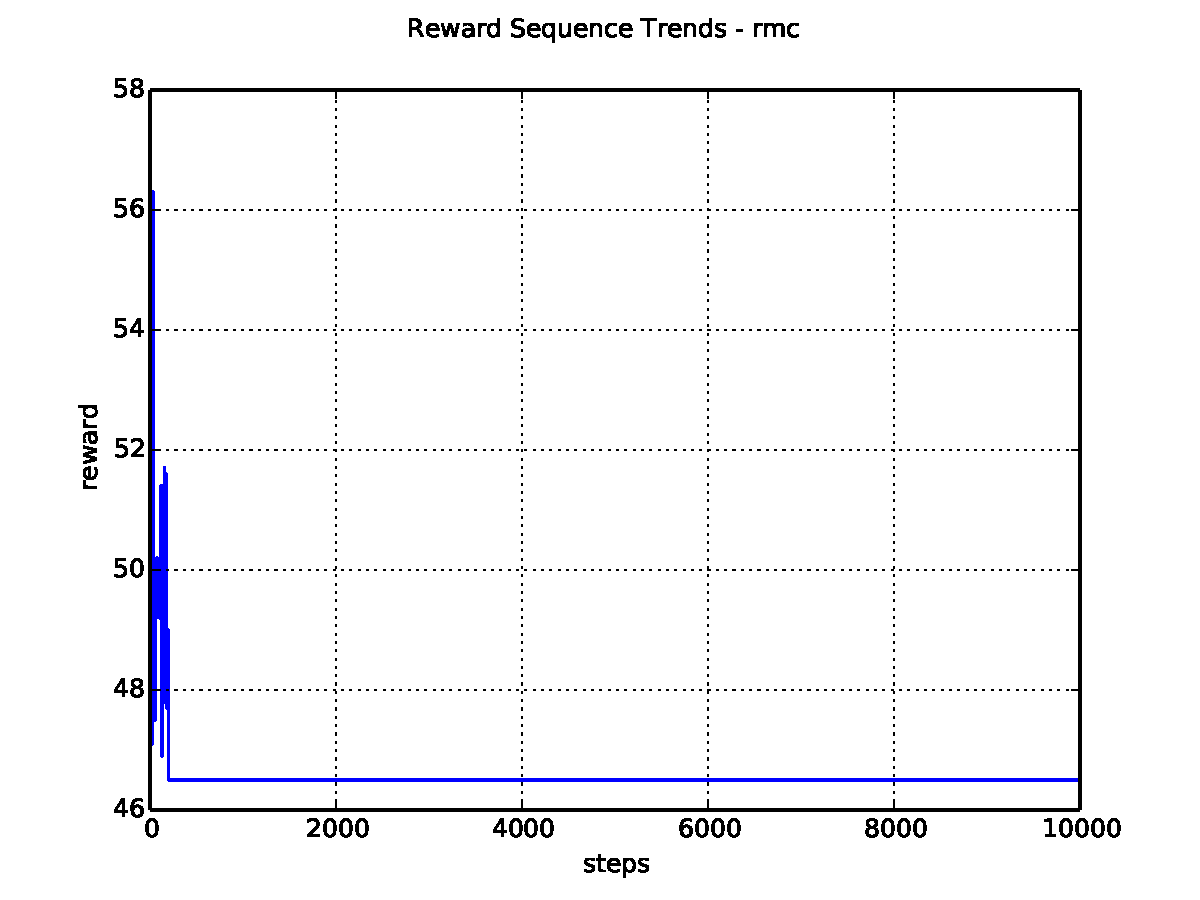
\includegraphics[width=0.8\textwidth]{trends_rmc.pdf}
\caption{\label{fig:trends_rmc}Trends of Reward Sequence for rmc}
\end{figure}  
\end{frame}

\begin{frame}
\begin{columns}
\column{.5\textwidth}
\begin{figure}[htb!]
\centering
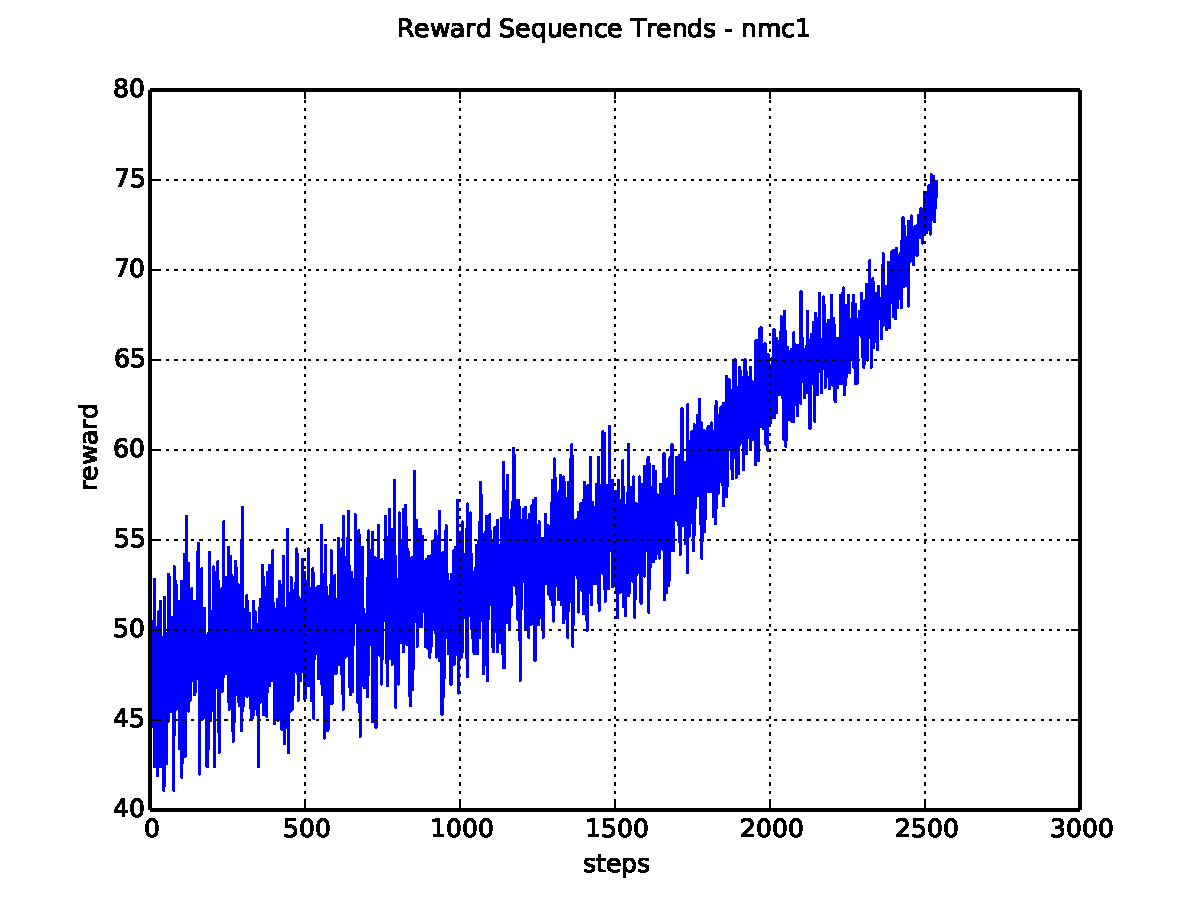
\includegraphics[width=1.0\textwidth]{trends_nmc1.pdf}
\caption{\label{fig:trends_nmc1}Trends of Reward Sequence for nmc1}
\end{figure}
\column{.5\textwidth}
\begin{figure}[htb!]
\centering
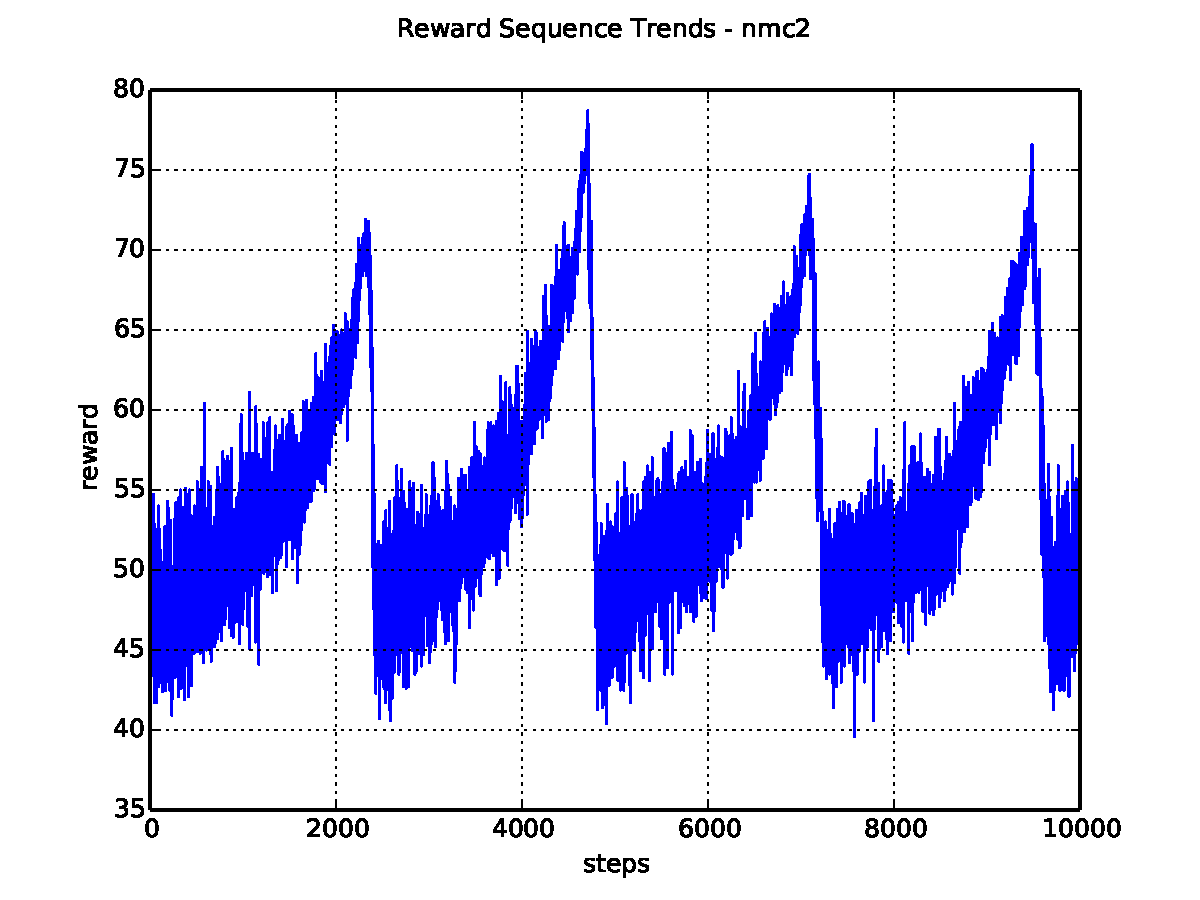
\includegraphics[width=1.0\textwidth]{trends_nmc2.pdf}
\caption{\label{fig:trends_nmc2}Trends of Reward Sequence for nmc2}
\end{figure}
\end{columns}
\end{frame}

\begin{frame}
\begin{columns}
\column{.5\textwidth}
\begin{figure}[htb!]
\centering
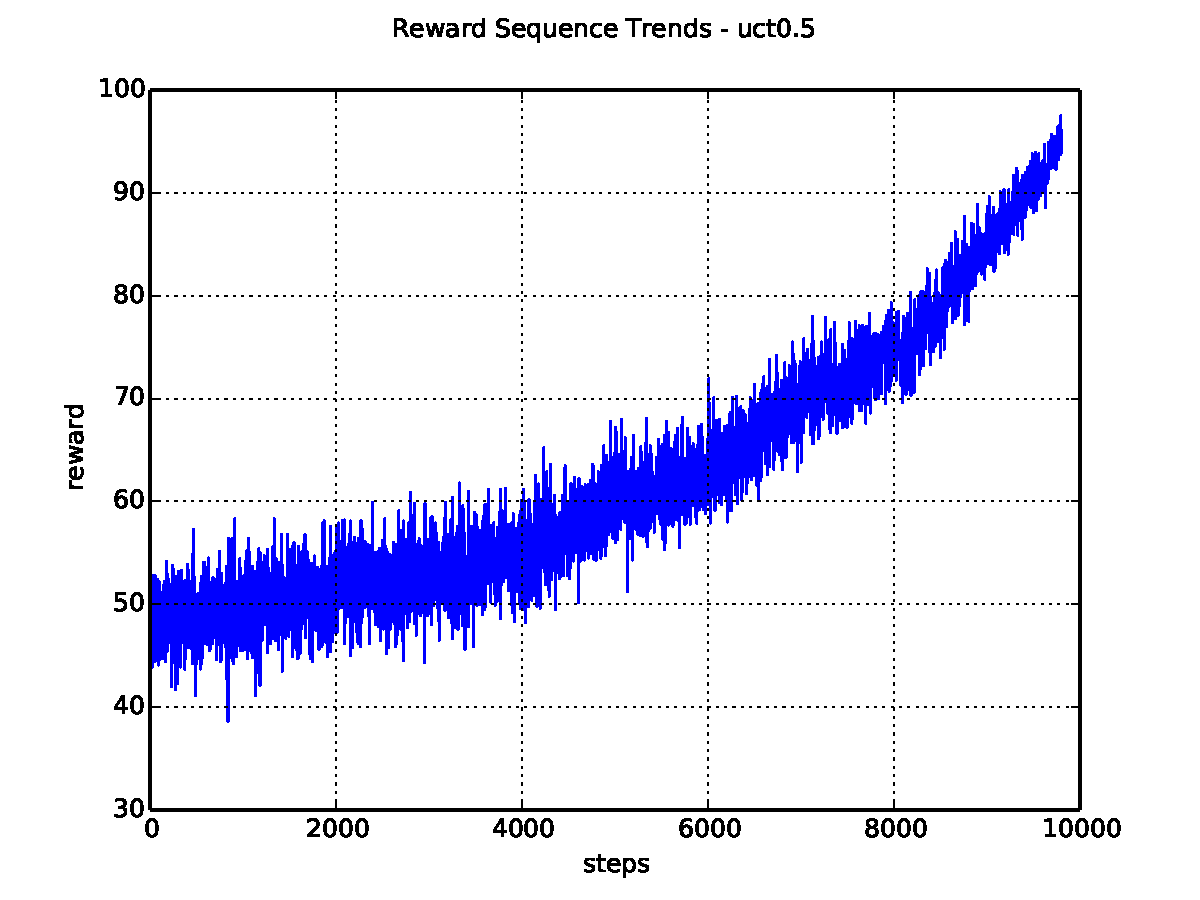
\includegraphics[width=1.0\textwidth]{trends_uct0_5.pdf}
\caption{\label{fig:trends_uct0.5}Trends of Reward Sequence for uct0.5}
\end{figure}
\column{.5\textwidth}
\begin{figure}[htb!]
\centering
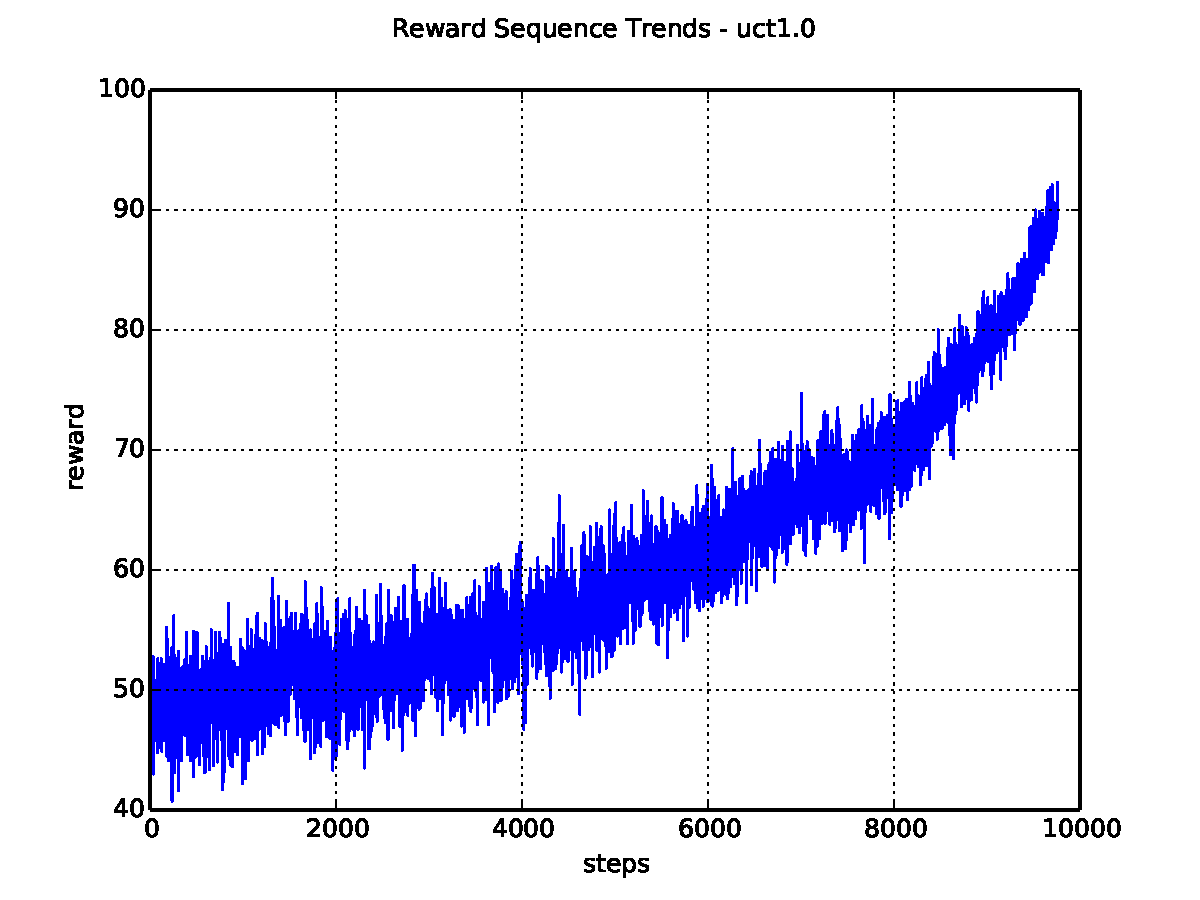
\includegraphics[width=1.0\textwidth]{trends_uct1_0.pdf}
\caption{\label{fig:trends_uct1.0}Trends of Reward Sequence for uct1.0}
\end{figure}
\end{columns}
\end{frame}

\subsection{Best Reward}

\begin{frame}
\begin{table}[htbp]
  \centering
  \caption{Best Reward}
    \begin{tabular}{cc}
    \toprule
    dataset & current best reward \\
    \midrule
    set 1 & 19 \\
    set 2 & 157 \\
    set 3 & 2612 \\
    set 4 & 248 \\
    set 5 & 1170 \\
    set 6 & 587 \\
    set 7 & 9979 \\
    \bottomrule
    \end{tabular}%
  \label{tab:best_rewards}%
\end{table}%xs
\end{frame}

\section{Conclusion}

\subsection{}

\begin{frame}
\begin{itemize}
  \item Summary
    \begin{itemize}
      \item uct0.5 and uct1.0 perform best in both criteria of optimality and efficiency among the five candidate algorithms
      \item uct seems like to learn the tree structure step by step 
      \item nmc1 is the most fast algorithm which can also guarantee a better soultion than rmc
    \end{itemize}
  \item Limitations
    \begin{itemize}
      \item More statistics should be stored for the deeper nodes.
      \item Randomly select a node to reduce the branching factor in the first layer.
      \item More deep understanding of the network and color sequence.
    \end{itemize}
\end{itemize}
\end{frame}

\begin{frame}
\Huge{\centerline{Thanks!}}
\centerline{Q\&A}
\end{frame}
\end{document} 
